\documentclass[11pt]{amsart}

\usepackage[T1]{fontenc}
\usepackage[sc,osf]{mathpazo}
\usepackage{amssymb}
\linespread{1.05}
\usepackage[margin=1.15in]{geometry}
\usepackage{microtype}
\usepackage{booktabs}
\usepackage{tikz}
\usetikzlibrary{arrows.meta,positioning,calc,shadows,fit,backgrounds}
\usepackage{pgfplots}
\pgfplotsset{compat=1.18}
\usepackage[hidelinks]{hyperref}
\makeatletter
\newcommand{\doi}{\begingroup\catcode`\_=12 \doi@}
\newcommand{\doi@}[1]{\href{https://doi.org/#1}{\nolinkurl{doi:#1}}\endgroup}
\makeatother
\usepackage[nameinlink]{cleveref}

\definecolor{ink}{HTML}{1F2A44}
\definecolor{sea}{HTML}{2E6F95}
\definecolor{sky}{HTML}{D8E8F3}
\definecolor{rust}{HTML}{B5532E}
\definecolor{sand}{HTML}{F6E7D8}
\definecolor{moss}{HTML}{4E7D4A}
\definecolor{leaf}{HTML}{E1EEDC}

\newtheorem{theorem}{Theorem}
\newtheorem{proposition}[theorem]{Proposition}
\newtheorem{lemma}[theorem]{Lemma}
\newtheorem{corollary}[theorem]{Corollary}
\theoremstyle{remark}
\newtheorem{remark}[theorem]{Remark}

\crefname{theorem}{Theorem}{Theorems}
\crefname{proposition}{Proposition}{Propositions}
\crefname{lemma}{Lemma}{Lemmas}
\crefname{corollary}{Corollary}{Corollaries}
\crefname{figure}{Figure}{Figures}
\crefname{table}{Table}{Tables}

\newcommand{\vp}{v_p}
\newcommand{\nO}{n_0}

\title{Wieferich Primes in Ordowski's Congruences}

\author{Deep}
\address{Independent researcher}
\email{dp.bh.in@gmail.com}

\subjclass[2020]{Primary 11A07; Secondary 11A51, 11Y11, 68V15}
\keywords{Wieferich prime, lifting the exponent, Carmichael function, largest prime exponent, formal verification}

\begin{document}

\begin{abstract}
We prove that no odd number with a repeated prime factor satisfies Ordowski's congruence for
every base, where the congruence asks that a base raised to the number and raised to its
largest prime exponent leave the same residue modulo the number. For the base two such
numbers do exist. Every prime carrying the largest exponent of one of them is a Wieferich
prime, and the smallest example is divisible by the square of 3511. Both answers are
verified in Lean.
\end{abstract}

\maketitle

\section{Introduction}

For a positive integer $n$ let $a(n)$ be the largest exponent in the prime factorization of
$n$, so that $a(1)=0$, $a(12)=2$ and $a(n)=1$ exactly when $n>1$ is squarefree. This is
sequence A051903 of the OEIS~\cite{oeis51903}. On 2 December 2019 Thomas Ordowski recorded
there three questions about this function.

\begin{enumerate}
\item[(Q1)] Is there a composite $n>4$ with $n\equiv a(n)\pmod{\varphi(n)}$?
\item[(Q2)] Is there an odd $n$ with $a(n)>1$ and $n\equiv a(n)\pmod{\lambda(n)}$?
\item[(Q3)] Is there an odd $n$ with $a(n)>1$ and $2^{n}\equiv 2^{a(n)}\pmod n$?
\end{enumerate}

Here $\varphi$ is Euler's function and $\lambda$ is Carmichael's function~\cite{carmichael}.
Ordowski added that a negative answer to (Q3) would give a negative answer to (Q2). The
first question is equivalent to Lehmer's totient problem~\cite{lehmer32}, an observation
recorded in the Formal Conjectures project~\cite{formalconj}, where all three questions are
stated in Lean and marked as open.\footnote{They appear there as
\texttt{OeisA51903.conjecture1}, \texttt{conjecture2} and \texttt{conjecture3}. The second is
stated in the equivalent form $b^n\equiv b^{a(n)}\pmod n$ for every $b$. The two forms agree
because $a(n)$ is at least every exponent of $n$, so both sides vanish modulo $p^{\vp(n)}$
whenever $p$ divides $b$, while for $b$ prime to $n$ the condition is $\lambda(n)\mid
n-a(n)$.}

We settle (Q2) and (Q3). Their answers differ, so the reduction noted by Ordowski does not
apply.

\begin{theorem}\label{thm:all}
No odd $n$ with $a(n)\ge 2$ satisfies $b^{n}\equiv b^{a(n)}\pmod n$ for every integer $b$.
More precisely, if $p$ is a prime with $p^{a(n)}\mid n$, then the base $b=p+1$ fails.
\end{theorem}

\begin{theorem}\label{thm:least}
The number
\[
\nO \;=\; 7\cdot 631\cdot 881\cdot 3511^{2}\cdot 201961 \;=\; 9687963167864344937
\]
satisfies $a(\nO)=2$ and $2^{\nO}\equiv 2^{2}\pmod{\nO}$. It is the least odd $n$ with
$a(n)>1$ and $2^{n}\equiv 2^{a(n)}\pmod n$.
\end{theorem}

Both theorems come from one inequality. If $p$ is an odd prime that attains the largest
exponent $E$ of $n$ and $b^{n}\equiv b^{E}\pmod{p^{E}}$, then lifting the exponent gives
$E\le\vp(b^{p-1}-1)+\vp(E)$ (\cref{prop:main}). Two consequences follow. The prime $p$ must be a base-$b$
Wieferich prime, which no prime is for the base $p+1$; this gives \cref{thm:all}. For the base
two it forces the square of $1093$ or $3511$ into every small witness, and a quadratic
residue argument removes $1093$. What remains is a search through numbers of the form
$3511^{2}m$, which produces $\nO$. \Cref{fig:map} shows the route.

Witnesses for the base two are plentiful once one is known: each one produces another from
a primitive prime divisor of a Mersenne number (\cref{cor:infinite}), and there are exactly
$28$ of them up to $3.49\cdot 10^{20}$ (\cref{thm:list}).

Everything in \cref{thm:all} and the first half of \cref{thm:least}, together with the
structural results of \cref{sec:base2}, has been verified in the Lean proof assistant
against the statements of the Formal Conjectures project. The minimality claim rests on a
computation that we describe in \cref{sec:least}.

\begin{figure}[t]
\centering
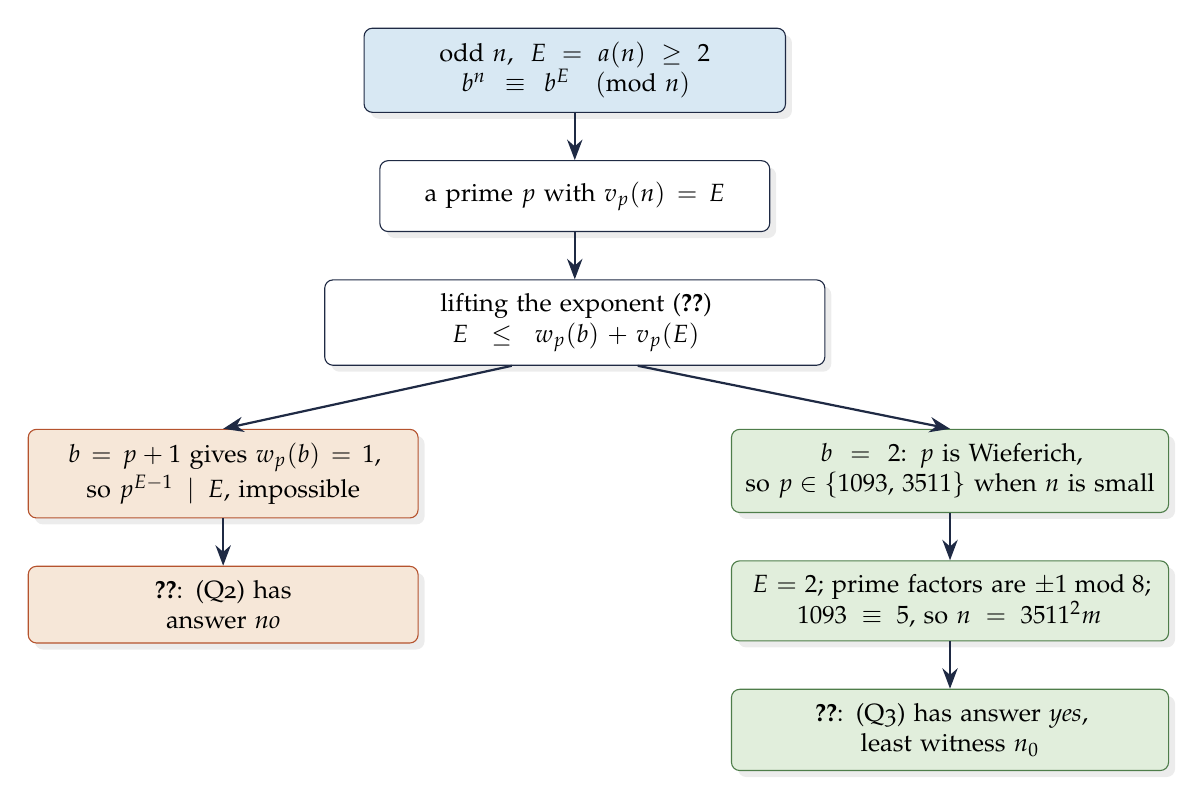
\begin{tikzpicture}[
  font=\small,
  box/.style={draw=ink, rounded corners=3pt, align=center, inner sep=5pt,
              minimum height=9mm, fill=white, drop shadow={opacity=0.15}},
  hyp/.style={box, fill=sky, text width=50mm},
  stp/.style={box, fill=white, text width=46mm},
  good/.style={box, fill=leaf, draw=moss, text width=52mm},
  bad/.style={box, fill=sand, draw=rust, text width=46mm},
  arr/.style={-{Stealth[length=2.6mm]}, thick, ink},
  node distance=6mm and 8mm]
  \node[hyp] (h) {odd $n$, \ $E=a(n)\ge 2$\\ $b^{n}\equiv b^{E}\pmod n$};
  \node[stp, below=of h] (p) {a prime $p$ with $\vp(n)=E$};
  \node[stp, below=of p, text width=60mm] (lte)
    {lifting the exponent (\cref{prop:main})\\ $E\le w_p(b)+\vp(E)$};
  \node[bad, below left=8mm and -12mm of lte] (b1)
    {$b=p+1$ gives $w_p(b)=1$,\\ so $p^{E-1}\mid E$, impossible};
  \node[good, below right=8mm and -12mm of lte] (b2)
    {$b=2$: $p$ is Wieferich,\\ so $p\in\{1093,\,3511\}$ when $n$ is small};
  \node[bad, below=of b1] (t1) {\textbf{\Cref{thm:all}}: (Q2) has\\ answer \emph{no}};
  \node[good, below=of b2] (c2) {$E=2$; prime factors are $\pm1 \bmod 8$;\\
     $1093\equiv 5$, so $n=3511^{2}m$};
  \node[good, below=of c2] (t2) {\textbf{\Cref{thm:least}}: (Q3) has answer \emph{yes},\\
     least witness $\nO$};
  \draw[arr] (h) -- (p);
  \draw[arr] (p) -- (lte);
  \draw[arr] (lte.south) ++(-8mm,0) -- (b1.north);
  \draw[arr] (lte.south) ++(8mm,0) -- (b2.north);
  \draw[arr] (b1) -- (t1);
  \draw[arr] (b2) -- (c2);
  \draw[arr] (c2) -- (t2);
\end{tikzpicture}
\caption{The structure of the argument. The left branch uses one base for each prime; the
right branch fixes the base two.}
\label{fig:map}
\end{figure}

\section{Lifting the exponent}\label{sec:lte}

For a prime $p$ and a nonzero integer $x$ we write $\vp(x)$ for the exponent of $p$ in $x$.
For an odd prime $p$ and an integer $b\ge 2$ prime to $p$ we put
\[
w_p(b)=\vp\bigl(b^{p-1}-1\bigr),
\]
which is at least $1$ by Fermat's theorem. The prime $p$ is a \emph{base-$b$ Wieferich prime}
if $w_p(b)\ge 2$. For $b=2$ these are the classical Wieferich primes~\cite{wieferich}; only
two are known, $1093$ and $3511$, and there are no others below $6.7\cdot
10^{15}$~\cite{doraisklyve}.\footnote{Earlier searches reached $6\cdot10^{9}$ (Lehmer
\cite{lehmer81}), $4\cdot 10^{12}$ (Crandall, Dilcher and Pomerance \cite{cdp}) and
$1.25\cdot10^{15}$ (Knauer and Richstein \cite{knauer}).} We write $w_p=w_p(2)$; a direct
computation gives $w_{1093}=w_{3511}=2$.

The following lemma is the classical lifting of the exponent; we include the short proof to
keep the paper self-contained.

\begin{lemma}\label{lem:lte}
Let $p$ be an odd prime, let $x\ge 2$ be an integer with $x\equiv 1\pmod p$, and let $k\ge
1$. Then $\vp(x^{k}-1)=\vp(x-1)+\vp(k)$.
\end{lemma}

\begin{proof}
If $p\nmid t$ then $(x^{t}-1)/(x-1)=1+x+\dots+x^{t-1}\equiv t\not\equiv 0\pmod p$, so
$\vp(x^{t}-1)=\vp(x-1)$. If $y=1+p^{r}u$ with $r\ge 1$ and $p\nmid u$, the binomial theorem
gives
\[
y^{p}=1+p^{r+1}u+\binom p2 p^{2r}u^{2}+\sum_{j\ge 3}\binom pj p^{jr}u^{j},
\]
and since $p$ is odd, $p\mid\binom p2$, so every term after the second is divisible by
$p^{r+2}$. Hence $\vp(y^{p}-1)=\vp(y-1)+1$. Writing $k=p^{s}t$ with $p\nmid t$ and applying
the second fact $s$ times to $y=x^{t}$ proves the lemma.
\end{proof}

\begin{proposition}\label{prop:main}
Let $p$ be an odd prime, let $b\ge 2$ be prime to $p$, and let $n\ge 1$ and $E\ge 1$ satisfy
$p^{E}\mid n$ and $b^{n}\equiv b^{E}\pmod{p^{E}}$. Then
\[
E\;\le\; w_p(b)+\vp(n-E)\;=\;w_p(b)+\vp(E).
\]
\end{proposition}

\begin{proof}
Since $n\ge p^{E}>E$, the integer $n-E$ is positive, and $\vp(E)<E\le\vp(n)$ gives
$\vp(n-E)=\vp(E)$. As $b$ is prime to $p$ we may cancel $b^{E}$ and obtain
$b^{\,n-E}\equiv 1\pmod{p^{E}}$. Raising to the power $p-1$ gives $x^{n-E}\equiv
1\pmod{p^{E}}$ with $x=b^{p-1}\equiv 1\pmod p$, and \cref{lem:lte} yields
\[
E\;\le\;\vp\bigl(x^{n-E}-1\bigr)\;=\;w_p(b)+\vp(n-E).\qedhere
\]
\end{proof}

\begin{corollary}\label{cor:wieferich}
Under the hypotheses of \cref{prop:main} with $E\ge 2$, the prime $p$ is a base-$b$
Wieferich prime.
\end{corollary}

\begin{proof}
If $w_p(b)=1$, then $\vp(E)\ge E-1$ by \cref{prop:main}, so $p^{E-1}\mid E$. But
$p^{E-1}\ge 3^{E-1}\ge 2E-1>E$ for $E\ge 2$.
\end{proof}

\Cref{fig:tower} pictures the mechanism. The units $x\equiv 1\pmod p$ form a descending
chain of layers according to $\vp(x-1)$, and raising to the power $k$ moves a unit up
exactly $\vp(k)$ layers. A witness must push $x=b^{p-1}$ to layer $E$, while the exponent
$n-E$ contributes exactly $\vp(E)$ layers.

\begin{figure}[t]
\centering
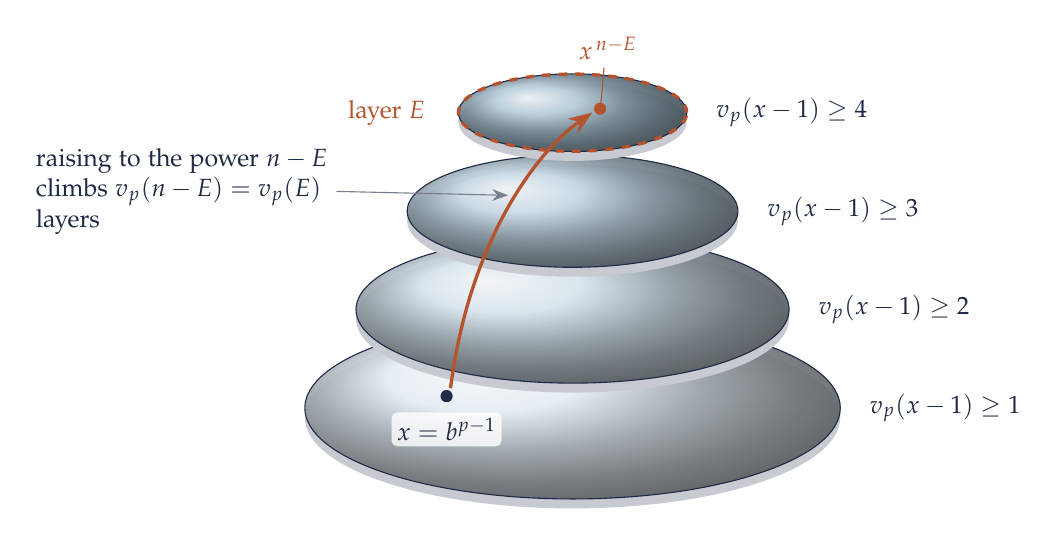
\begin{tikzpicture}[font=\small, x=1cm, y=1cm]
  % stacked discs: layer k = { x : v_p(x-1) >= k }
  \foreach \k/\r/\c in {1/3.4/sky, 2/2.75/sky!85!sea, 3/2.1/sky!65!sea, 4/1.45/sky!45!sea} {
    \pgfmathsetmacro{\h}{1.25*(\k-1)}
    \fill[ink!25] (0,\h-0.12) ellipse ({\r} and {0.34*\r});
    \shade[ball color=\c!70!white, opacity=0.9] (0,\h) ellipse ({\r} and {0.34*\r});
    \draw[ink, thin] (0,\h) ellipse ({\r} and {0.34*\r});
    \node[anchor=west, ink] at (\r+0.25,\h) {$\vp(x-1)\ge \k$};
  }
  % the target layer E
  \draw[rust, very thick, dashed] (0,3.75) ellipse (1.45 and 0.49);
  \node[rust, anchor=east] at (-1.75,3.75) {layer $E$};
  % points
  \fill[ink] (-1.6,0.15) circle (2.2pt);
  \node[anchor=north, ink, fill=white, fill opacity=0.8, text opacity=1,
        rounded corners=2pt, inner sep=2pt] at (-1.6,-0.05) {$x=b^{p-1}$};
  \fill[rust] (0.35,3.8) circle (2.2pt);
  \node[anchor=south, rust] at (0.45,4.3) {$x^{\,n-E}$};
  \draw[rust, thin] (0.4,4.32) -- (0.36,3.86);
  \draw[-{Stealth[length=3mm]}, very thick, rust]
    (-1.55,0.25) .. controls (-1.3,2.2) and (-0.4,3.3) .. (0.25,3.75);
  \node[align=left, anchor=east, ink, fill=white, fill opacity=0.9, text opacity=1,
        rounded corners=2pt, inner sep=3pt] (lab) at (-3.0,2.75)
    {raising to the power $n-E$\\ climbs $\vp(n-E)=\vp(E)$\\ layers};
  \draw[ink!60, thin, -{Stealth[length=2mm]}] (lab.east) -- (-0.82,2.7);
\end{tikzpicture}
\caption{The layers $\{x\equiv 1\pmod{p^{k}}\}$ drawn as stacked discs. A unit on layer
$w_p(b)$ reaches layer $E$ only if $E\le w_p(b)+\vp(E)$; for $E\ge2$ this needs
$w_p(b)\ge2$.}
\label{fig:tower}
\end{figure}

\section{Every base at once}\label{sec:all}

\begin{proof}[Proof of \cref{thm:all}]
Let $n$ be odd with $E=a(n)\ge 2$, and choose a prime $p$ with $\vp(n)=E$. It is odd
because $n$ is. Put $b=p+1$, which is prime to $p$. By \cref{lem:lte} applied to $x=p+1$ and
$k=p-1$,
\[
w_p(p+1)=\vp\bigl((p+1)^{p-1}-1\bigr)=\vp(p)+\vp(p-1)=1.
\]
So $p$ is not a base-$(p+1)$ Wieferich prime. If $b^{n}\equiv b^{E}\pmod n$, the same holds
modulo $p^{E}$, and \cref{cor:wieferich} gives a contradiction.
\end{proof}

\begin{remark}
In the language of (Q2) the proof says that $p^{E-1}$, which divides $\lambda(n)$, cannot
divide $n-E$. This is the same mechanism that reduces (Q1) to Lehmer's problem in
\cite{formalconj}. The point of \cref{prop:main} is that it records what a single base
forces, and this is what the question for the base two requires.
\end{remark}

\section{The base two}\label{sec:base2}

From now on a \emph{witness} is an odd $n$ with $a(n)\ge 2$ and $2^{n}\equiv
2^{a(n)}\pmod n$.

\begin{theorem}\label{thm:shape}
Let $n$ be a witness and $E=a(n)$.
\begin{enumerate}
\item Every prime $p$ with $\vp(n)=E$ is a Wieferich prime, and $E\le w_p+\vp(E)$.
\item If $E$ is even, every prime factor $q$ of $n$ satisfies $q\equiv\pm1\pmod 8$.
\item If every prime $p$ with $\vp(n)=E$ is below $6.7\cdot 10^{15}$, which holds in
particular when $n<4.4\cdot 10^{31}$, then $E=2$ and
\[
n=3511^{2}m,\qquad m \text{ squarefree},\qquad 3511\nmid m,\qquad m\equiv 1757\pmod{3510}.
\]
\end{enumerate}
\end{theorem}

\begin{proof}
Part (1) is \cref{prop:main} and \cref{cor:wieferich} with $b=2$.

For (2), let $q$ be a prime factor of $n$; it is odd. Cancelling $2^{E}$ gives
$2^{n-E}\equiv1\pmod q$, and $n-E=2k+1$ is odd. Hence $2\equiv 2^{2k+2}=(2^{k+1})^{2}\pmod
q$, so $2$ is a quadratic residue modulo $q$, which happens exactly when $q\equiv\pm1\pmod
8$~\cite[Ch.~5]{irelandrosen}.

For (3), each prime $p$ with $\vp(n)=E$ is a Wieferich prime below $6.7\cdot10^{15}$ by (1),
so $p\in\{1093,3511\}$ by \cite{doraisklyve}, and $w_p=2$. If $E\ge3$ then $p^{E-2}\mid E$
by (1), which is impossible since $p^{E-2}\ge 1093^{E-2}>E$. Thus $E=2$. Now every prime whose square divides $n$
attains the exponent $E$, so it is $1093$ or $3511$. Part (2) applies because $E$ is even,
and $1093\equiv 5\pmod 8$, so $1093\nmid n$. Hence $n=3511^{2}m$ with $m$ squarefree and
prime to $3511$. The order of $2$ modulo $3511^{2}$ is $1755=3^{3}\cdot5\cdot13$, the same as
modulo $3511$; one checks that $2^{1755}\equiv1\pmod{3511^{2}}$ and that $2^{1755/r}\not\equiv
1\pmod{3511}$ for $r=3,5,13$. From $2^{n-2}\equiv1\pmod{3511^{2}}$ we get $1755\mid
3511^{2}m-2$, and since $3511\equiv1\pmod{1755}$ this says $m\equiv2\pmod{1755}$. As $m$ is
odd, $m\equiv1757\pmod{3510}$.
\end{proof}

\begin{table}[t]
\centering
\caption{The prime power factors of $\nO$. Each order divides
$19305=3^{3}\cdot5\cdot11\cdot13$, and $\nO\equiv 2\pmod{19305}$.}
\label{tab:n0}
\begin{tabular}{@{}rccc@{}}
\toprule
$q^{e}$ & $q \bmod 8$ & order of $2$ modulo $q^{e}$ & where $q$ comes from\\
\midrule
$7$ & $7$ & $3$ & $2^{3}-1$\\
$631$ & $7$ & $45=3^{2}\cdot5$ & $2^{45}-1$\\
$881$ & $1$ & $55=5\cdot11$ & $2^{55}-1$\\
$3511^{2}$ & $7$ & $1755=3^{3}\cdot5\cdot13$ & Wieferich\\
$201961$ & $1$ & $55=5\cdot11$ & $2^{55}-1$\\
\bottomrule
\end{tabular}
\end{table}

\begin{proof}[Proof that $\nO$ is a witness]
The factorization of $\nO$ shows $a(\nO)=2$. For each prime power $q^{e}\,\|\,\nO$,
\cref{tab:n0} lists the order of $2$ modulo $q^{e}$. All of these orders divide $19305$, and
$\nO-2=19305\cdot 501836993932367$, so $2^{\nO-2}\equiv1$ modulo every $q^{e}$ and hence
modulo $\nO$. Multiplying by $4$ gives $2^{\nO}\equiv 2^{2}\pmod{\nO}$.
\end{proof}

The table explains how $\nO$ was found. Once $3511^{2}$ is fixed, it is natural to look for
$m$ among products of primes $q$ whose order $\operatorname{ord}_q(2)$ divides a small multiple
$L$ of $1755$. Then the only remaining condition is $3511^{2}m\equiv2\pmod L$, a congruence
on a product of residues. With $L=19305$ the primes dividing $2^{d}-1$ for $d\mid L$ already
contain the solution above.\footnote{The first witness we found this way was
$3511^{2}\cdot7\cdot31\cdot73\cdot79\cdot89\cdot271\cdot937=348634396442820771857$.}

\begin{corollary}\label{cor:infinite}
If $n$ is a witness with $a(n)=2$ and $q$ is a prime with $\operatorname{ord}_q(2)=n-2$, then
$nq$ is a witness with $a(nq)=2$. Consequently there are infinitely many witnesses.
\end{corollary}

\begin{proof}
Since $n-2=\operatorname{ord}_q(2)$ divides $q-1$, and $q\ne n-1$ because $n-1$ is even, we
have $q\ge 2(n-2)+1>n$. So $q$ is odd and $q\nmid n$; thus $nq$ is odd and $a(nq)=2$. Modulo $q$, the exponent $nq-2=(n-2)q+2(q-1)$ is a
multiple of $n-2$. Modulo $n$, the order of $2$ divides $n-2$, which divides $q-1$, and
$nq-2=n(q-1)+(n-2)$. Hence $2^{nq-2}\equiv1\pmod{nq}$. A prime $q$ with
$\operatorname{ord}_q(2)=n-2$ exists by Zsigmondy's theorem~\cite{zsigmondy}, so starting
from $\nO$ the construction never stops.
\end{proof}

\section{The least witness}\label{sec:least}

\begin{proof}[Proof that $\nO$ is the least witness]
Let $n\le\nO$ be a witness. Every prime $p$ with $\vp(n)=a(n)$ satisfies $p^{2}\le n$, so
$p<3.12\cdot 10^{9}$. We tested every prime below $4.2\cdot10^{9}$ and found that
$1093$ and $3511$ are the only Wieferich primes in this range, in agreement
with~\cite{lehmer81,cdp}. The argument for part~(3) of \cref{thm:shape} then applies
verbatim, so $n=3511^{2}m$ with
\[
m\equiv1757\pmod{3510},\qquad m\equiv\pm1\pmod 8,\qquad 3511\nmid m,\qquad
2^{3511^{2}m-2}\equiv1\pmod m .
\]
The second condition comes from part~(2) of \cref{thm:shape}, and the last is the witness
condition modulo $m$. We enumerated all $m\le 785906390297$ in these two residue classes
modulo $14040$, about $1.12\cdot 10^{8}$ values, and computed $2^{3511^{2}m-2}\bmod m$ with
Montgomery multiplication. The first value satisfying the congruence conditions is
$m=785906390297=7\cdot631\cdot881\cdot201961$, which is squarefree and gives $n=\nO$.
\end{proof}

The same search, run up to $m\le 28281899434817$, finds every witness up to
\[
N_1=3511^{2}\cdot 28281899434817=348634396442820771857\approx 3.49\cdot10^{20}.
\]

\begin{theorem}\label{thm:list}
There are exactly $28$ witnesses $n\le N_1$. All of them have $a(n)=2$ and the form
$3511^{2}m$ with $m$ squarefree; they are listed in \cref{tab:list}.
\end{theorem}

\begin{proof}
For a witness $n\le N_1$, the primes attaining $a(n)$ lie below $\sqrt{N_1}<1.9\cdot10^{10}$,
a range in which $1093$ and $3511$ are the only Wieferich primes~\cite{cdp}. As in the
previous proof, $n=3511^{2}m$ with $m$ in the two residue classes modulo $14040$ and
$m\le 28281899434817$. All $4.03\cdot10^{9}$ such $m$ were tested. The $28$ values that
satisfy the congruence were then checked again in exact integer arithmetic; each is
squarefree, prime to $3511$, and gives $2^{n}\equiv4\pmod n$.
\end{proof}

The largest entry of \cref{tab:list} is the first witness we found by the construction above.
\Cref{fig:witnesses} shows how the witnesses spread out.

\begin{table}[t]
\centering
\small
\caption{All witnesses $n=3511^{2}m\le 348634396442820771857$, with the prime factors of
$m$.}
\label{tab:list}
\begin{tabular}{@{}rrl@{}}
\toprule
& $n$ & $m$\\
\midrule
1 & $9687963167864344937$ & $7\cdot 631\cdot 881\cdot 201961$\\
2 & $10191389002728947327$ & $439\cdot 631\cdot 1151\cdot 2593$\\
3 & $11613371395592377127$ & $23\cdot 73\cdot 89\cdot 1327\cdot 4751$\\
4 & $12853981953529455377$ & $71\cdot 73\cdot 79\cdot 751\cdot 3391$\\
5 & $12874928605806902897$ & $31\cdot 79\cdot 151\cdot 431\cdot 6553$\\
6 & $13730896205770900457$ & $7\cdot 31\cdot 271\cdot 18941231$\\
7 & $15996167795452598327$ & $7\cdot 79\cdot 23279\cdot 100801$\\
8 & $18091379716837511177$ & $127\cdot 20231\cdot 571201$\\
9 & $21095218232071695857$ & $23\cdot 151\cdot 6553\cdot 75193$\\
10 & $29350506332796150647$ & $73\cdot 79\cdot 89\cdot 199\cdot 23311$\\
11 & $39992485447538478857$ & $71\cdot 199\cdot 263\cdot 881\cdot 991$\\
12 & $67350552227362140167$ & $73\cdot 191\cdot 199\cdot 1969111$\\
13 & $73657883659512951047$ & $311\cdot 16183\cdot 1187239$\\
14 & $82340163204173730767$ & $79\cdot 36793\cdot 2298041$\\
15 & $98848358486672333177$ & $71\cdot 73\cdot 151\cdot 1801\cdot 5689$\\
16 & $139478761055861260607$ & $7\cdot 89\cdot 151\cdot 991\cdot 121369$\\
17 & $161001183676264892417$ & $47\cdot 71\cdot 487\cdot 599\cdot 13417$\\
18 & $164739335550634207937$ & $7\cdot 89\cdot 1567\cdot 2089\cdot 6553$\\
19 & $191711593813855690577$ & $79\cdot 4201\cdot 6553\cdot 7151$\\
20 & $201401736552101605457$ & $7\cdot 103\cdot 311\cdot 6553\cdot 11119$\\
21 & $204945450678447017177$ & $45137\cdot 368335801$\\
22 & $223934360665868890247$ & $7\cdot 31\cdot 66161\cdot 1265311$\\
23 & $225021378651588304697$ & $73\cdot 79\cdot 151\cdot 271\cdot 77351$\\
24 & $259428933707962157687$ & $71\cdot 911\cdot 2647\cdot 122921$\\
25 & $275690737952807302127$ & $71\cdot 751\cdot 881\cdot 476087$\\
26 & $316763115741760627487$ & $31\cdot 631\cdot 10687\cdot 122921$\\
27 & $324284460815828474327$ & $271\cdot 337\cdot 11471\cdot 25111$\\
28 & $348634396442820771857$ & $7\cdot 31\cdot 73\cdot 79\cdot 89\cdot 271\cdot 937$\\
\bottomrule
\end{tabular}
\end{table}

\begin{figure}[t]
\centering
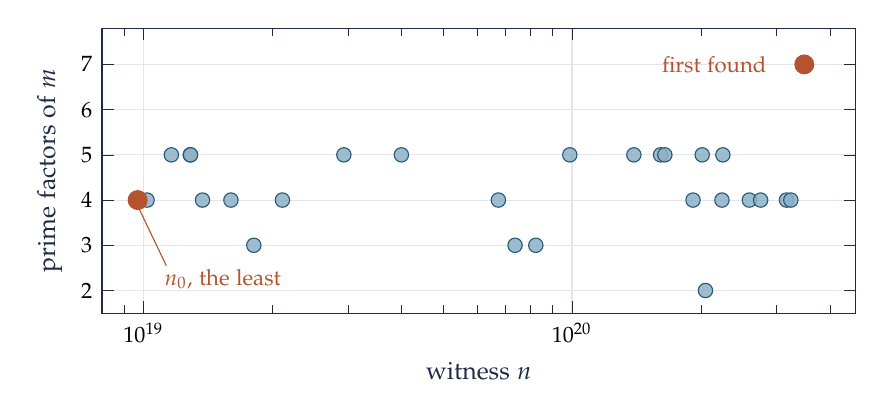
\begin{tikzpicture}
\begin{axis}[
  width=0.92\textwidth, height=5.2cm,
  xmode=log, xmin=8e18, xmax=4.6e20,
  ymin=1.5, ymax=7.8, ytick={2,3,4,5,6,7},
  xlabel={witness $n$}, ylabel={prime factors of $m$},
  axis line style={ink}, tick style={ink}, label style={ink, font=\small},
  ticklabel style={font=\footnotesize},
  grid=major, grid style={ink!12},
  clip=false]
\addplot[only marks, mark=*, mark size=2.6pt, draw=sea!80!black, fill=sea!55,
  fill opacity=0.85] coordinates {(9.687963e+18,4) (1.019139e+19,4) (1.161337e+19,5) (1.285398e+19,5) (1.287493e+19,5) (1.373090e+19,4) (1.599617e+19,4) (1.809138e+19,3) (2.109522e+19,4) (2.935051e+19,5) (3.999249e+19,5) (6.735055e+19,4) (7.365788e+19,3) (8.234016e+19,3) (9.884836e+19,5) (1.394788e+20,5) (1.610012e+20,5) (1.647393e+20,5) (1.917116e+20,4) (2.014017e+20,5) (2.049455e+20,2) (2.239344e+20,4) (2.250214e+20,5) (2.594289e+20,4) (2.756907e+20,4) (3.167631e+20,4) (3.242845e+20,4) (3.486344e+20,7)};
\addplot[only marks, mark=*, mark size=3.4pt, draw=rust, fill=rust]
  coordinates {(9.687963e+18,4) (3.486344e+20,7)};
\draw[rust, thin] (axis cs:9.75e+18,3.82) -- (axis cs:1.13e+19,2.55);
\node[anchor=north west, rust, font=\footnotesize, inner sep=1pt]
  at (axis cs:1.10e+19,2.55) {$\nO$, the least};
\node[anchor=east, rust, font=\footnotesize, align=right]
  at (axis cs:3.0e+20,7) {first found};
\end{axis}
\end{tikzpicture}
\caption{The $28$ witnesses up to $N_1$, by size and by the number of prime factors of $m$.
Every one of them is divisible by $3511^{2}$.}
\label{fig:witnesses}
\end{figure}

\section{Formal verification}\label{sec:lean}

The file \texttt{ErdosProofs/Ordowski.lean} in the accompanying repository~\cite{repo}
proves the following in Lean~4~\cite{lean4} with Mathlib~\cite{mathlib}.\footnote{We
used Lean v4.33.0 with Mathlib v4.33.0. The definition of $a$ is copied verbatim from the
statement in~\cite{formalconj}.}

\begin{itemize}
\item \texttt{conjecture2}: the statement of (Q2) from~\cite{formalconj} with answer
\texttt{False} (\cref{thm:all}).
\item \texttt{conjecture3}: the statement of (Q3) with answer \texttt{True}, using the witness
$\nO$.
\item \texttt{le\_padicValNat\_of\_modEq} and \texttt{wieferich\_of\_modEq}: the inequality
$E\le w_p(b)+\vp(n-E)$ of \cref{prop:main} and \cref{cor:wieferich}, for every base.
\item \texttt{base\_two\_wieferich} and \texttt{prime\_factor\_mod\_eight}: parts (1) and
(2) of \cref{thm:shape}.
\end{itemize}

Lifting the exponent is Mathlib's \texttt{padicValNat.pow\_sub\_pow}, and the quadratic
character of $2$ is \texttt{ZMod.exists\_sq\_eq\_two\_iff}. The congruence
$2^{\nO}\equiv4\pmod{\nO}$ cannot be checked by expanding $2^{\nO}$, which has about
$10^{19}$ binary digits. Instead the file defines binary modular exponentiation, proves that
it computes $b^{e}\bmod m$, and lets the kernel evaluate it in sixty-four squaring steps. The
factorization of $\nO$ is certified by Mathlib's \texttt{norm\_num} primality extension. No
step uses \texttt{native\_decide}, so the proofs rely only on the Lean kernel and the
standard axioms \texttt{propext}, \texttt{Classical.choice} and \texttt{Quot.sound}. The
search behind \cref{sec:least} is not formalized; its C source is in the repository.

\section*{Acknowledgments}
The author thanks Thomas Ordowski for posing these questions and the Formal Conjectures
team for stating them in Lean. Claude, an AI model developed by Anthropic, assisted with
the computations, the Lean formalization and the preparation of the manuscript.

\begin{thebibliography}{99}

\bibitem{carmichael}
R.~D. Carmichael, \emph{Note on a new number theory function}, Bull. Amer. Math. Soc.
\textbf{16} (1910), 232--238. \doi{10.1090/S0002-9904-1910-01892-9}

\bibitem{cdp}
R.~Crandall, K.~Dilcher and C.~Pomerance, \emph{A search for Wieferich and Wilson primes},
Math. Comp. \textbf{66} (1997), 433--449. \doi{10.1090/S0025-5718-97-00791-6}

\bibitem{doraisklyve}
F.~G. Dorais and D.~Klyve, \emph{A Wieferich prime search up to $6.7\times10^{15}$}, J.
Integer Seq. \textbf{14} (2011), Article 11.9.2.

\bibitem{formalconj}
Google DeepMind, \emph{Formal Conjectures}, file
\texttt{FormalConjectures/OEIS/51903.lean},
\url{https://github.com/google-deepmind/formal-conjectures}.

\bibitem{irelandrosen}
K.~Ireland and M.~Rosen, \emph{A Classical Introduction to Modern Number Theory}, 2nd ed.,
Grad. Texts in Math. \textbf{84}, Springer, New York, 1990.
\doi{10.1007/978-1-4757-2103-4}

\bibitem{knauer}
J.~Knauer and J.~Richstein, \emph{The continuing search for Wieferich primes}, Math. Comp.
\textbf{74} (2005), 1559--1563. \doi{10.1090/S0025-5718-05-01723-0}

\bibitem{lehmer32}
D.~H. Lehmer, \emph{On Euler's totient function}, Bull. Amer. Math. Soc. \textbf{38} (1932),
745--751. \doi{10.1090/S0002-9904-1932-05521-5}

\bibitem{lehmer81}
D.~H. Lehmer, \emph{On Fermat's quotient, base two}, Math. Comp. \textbf{36} (1981),
289--290. \doi{10.1090/S0025-5718-1981-0595064-5}

\bibitem{mathlib}
The mathlib Community, \emph{The Lean mathematical library}, in: Proceedings of the 9th ACM
SIGPLAN International Conference on Certified Programs and Proofs (CPP 2020), ACM, 2020,
367--381. \doi{10.1145/3372885.3373824}

\bibitem{lean4}
L.~de~Moura and S.~Ullrich, \emph{The Lean 4 theorem prover and programming language}, in:
Automated Deduction, CADE~28, Lecture Notes in Comput. Sci. \textbf{12699}, Springer, 2021,
625--635. \doi{10.1007/978-3-030-79876-5_37}

\bibitem{oeis51903}
OEIS Foundation Inc., \emph{Sequence A051903}, The On-Line Encyclopedia of Integer
Sequences, \url{https://oeis.org/A051903}.

\bibitem{repo}
Deep, \emph{Erodos-breakthrough}, source code and Lean proofs,
\url{https://github.com/creelie/Erodos-breakthrough}.

\bibitem{wieferich}
A.~Wieferich, \emph{Zum letzten Fermat'schen Theorem}, J. Reine Angew. Math. \textbf{136}
(1909), 293--302. \doi{10.1515/crll.1909.136.293}

\bibitem{zsigmondy}
K.~Zsigmondy, \emph{Zur Theorie der Potenzreste}, Monatsh. Math. Phys. \textbf{3} (1892),
265--284. \doi{10.1007/BF01692444}

\end{thebibliography}

\end{document}
